% !TEX root = ../thesis.tex

\chapter{Syncer Optimisations}
\label{cha:optimisations}
In this chapter, we improve on the initial design of the framework described in chapter \ref{cha:design_implementation}. We run benchmarks on the optimisations proposed, and present the results. The specifications of the two setups used for testing are shown in table \ref{table:benchmark-specs}.

\begin{table}[H]
  \centering
  \begin{adjustbox}{max width=1.2\textwidth, center}
    \begin{subtable}{0.5\textwidth}
      \begin{tabular}{|r|l|} \hline
        \multicolumn{2}{|c|}{\textbf{MacBook Pro 2011}} \\ \hline
        \textbf{Operating System} & OS X 10.10.4 (Yosemite)\\ \hline
        \textbf{Processor} & 2.3 GHz Intel Core i5\\ \hline
        \textbf{Memory} & 8 GB 1333 MHz DDR3 \\ \hline
        \textbf{Storage} & 256GB SSD Crucial m4\\ \hline
        \textbf{Network Speed} & 24.4/2.5 Mbit/s\\ \hline
      \end{tabular}
      \caption{MBP}
    \end{subtable}

    \begin{subtable}{0.5\textwidth}
      \begin{tabular}{|r|l|} \hline
        \multicolumn{2}{|c|}{\textbf{\textasciitilde okeanos Virtual Machine}}
        \\ \hline
        \textbf{Operating System} & Ubuntu Linux 14.04.2 LTS (Trusty)\\ \hline
        \textbf{Processor} & 2.1 GHz Virtual CPU QEMU v2.1.2 \\ \hline
        \textbf{Memory} & 4 GB Virtual RAM \\ \hline
        \textbf{Storage} & 80 GB (DRBD) \\ \hline
        \textbf{Network Speed} & 344.6/137.3 Mbit/s\\ \hline
      \end{tabular}
      \caption{VM}
    \end{subtable}
  \end{adjustbox}
  \caption{Benchmark setups specs}
  \label{table:benchmark-specs}
\end{table}

\section{Request queuing}
  After using the framework with the help of a profiler, it became apparent that a bottleneck existed whenever there was a need for multiple requests on the remote server, due to the latency and the round-trip times. Additionally, during the transfer (download or upload) of a large file, the synchronisation process was being unnecessarily stalled until the tranfer finished. To overcome these issues, a request queuing system was implemented, dispatching the requests to different threads, while the main thread continued the execution of the sync. There was also a dramatic speedup when step 2 of the syncing algorithm was modified to request all objects' metadata from the remote server together, instead of individually for each file. To ensure correctness in the synchronisation process, the program should wait until all threads executing requests for a step of an algorithm (as described in section \ref{ssec:3step_algorithm}) have finished, before starting a different step. A more efficient solution would be to implement a locking mechanism and disallow actions on files already being processed by a spawned thread, but this would require substantial changes in the framework code.
  \subsection{Benchmarks}
    \subsubsection{Upload time relative to number of threads}
      For the first benchmark, we tried to upload 100 files of 150 bytes each sequentially (denoted as ``0'' threads in table \ref{table:upload-threads}) and again by using a different number of threads. The files were always being randomly generated, because Pithos+ stores the blocks that are uploaded, and we needed to evade that caching for accurate measurements. Each batch of uploads was executed 10 times, and the results presented are the average of those tries. The results are statistically accurate, having a standard deviation of $\sigma_A = 1.1$.
      \begin{table}[H]
        \setlength{\tabcolsep}{12pt}
        \begin{subtable}{\textwidth}
          \begin{adjustbox}{max width=1.2\textwidth, center}
          \begin{tabular}{c|*{12}{c|}}
            \cline{2-12}
            & \multicolumn{11}{ |c| }{\textbf{\# of threads}} \\ \cline{2-12}
            & \textbf{0} & \textbf{1} & \textbf{2} & \textbf{4} & \textbf{8} & \textbf{12} & \textbf{16} & \textbf{20} & \textbf{24} & \textbf{28} & \textbf{32} \\ \cline{1-12}
            \multicolumn{1}{ |c| }{\textbf{time (s)}} & 92.55 & 91.51 & 48.33 & 33.42 & 29.79 & 29.80 & 30.85 & 30.79 & 30.95 & 30.68 & 31.23 \\ \cline{1-12}
            \multicolumn{1}{ |c| }{\textbf{speedup (\%)}} & N/A & 1.51 & 47.78 &  63.89 & 67.81 & 67.80 & 66.67 & 66.73 & 66.56 & 66.85 & 66.25 \\ \cline{1-12}
          \end{tabular}
          \end{adjustbox}
          \caption{MBP}
        \end{subtable}

        \begin{subtable}{\textwidth}
          \begin{adjustbox}{max width=1.2\textwidth, center}
          \begin{tabular}{c|*{12}{c|}}
            \cline{2-12}
            & \multicolumn{11}{ |c| }{\textbf{\# of threads}} \\ \cline{2-12}
            & \textbf{0} & \textbf{1} & \textbf{2} & \textbf{4} & \textbf{8} & \textbf{12} & \textbf{16} & \textbf{20} & \textbf{24} & \textbf{28} & \textbf{32} \\ \cline{1-12}
            \multicolumn{1}{ |c| }{\textbf{time (s)}} & 76.24 & 72.79 & 43.92 & 33.82 & 29.90 & 33.52 & 34.85 & 33.18 & 33.01 & 33.98 & 32.26 \\ \cline{1-12}
            \multicolumn{1}{ |c| }{\textbf{speedup (\%)}} & N/A & -0.21 & 39.54 & 53.44 & 58.84 & 53.85 & 52.03 & 54.31 & 54.55 & 53.21 & 55.58 \\ \cline{1-12}
          \end{tabular}
          \end{adjustbox}
          \caption{VM}
        \end{subtable}
        \caption{Upload speedup by queuing, relative to \# of threads}
        \label{table:upload-threads}
      \end{table}

      As seen in table \ref{table:upload-threads}, there is a considerable speedup when using multiple threads to upload the files, with the uploads completing in less than half the time on the VM, when 4 or more threads were used. It is worth mentioning that the pithos service used raised exceptions on some requests when using 8 or more threads. Since reliability is a core element of a synchronisation framework, the use of 4 or less threads is recommended when using this feature.

      \begin{table}[H]
        \begin{adjustbox}{max width=1.2\textwidth, center}
        \begin{subtable}{0.6\textwidth}
          \centering
          \begin{adjustbox}{max width=.95\textwidth, center}
          \begin{tabular}{c|*{4}{c|}}
            \cline{2-4}
            & \multicolumn{3}{ |c| }{\textbf{File Size}} \\ \cline{2-4}
            & \textbf{150 B} & \textbf{150 KB} & \textbf{1.5 MB} \\ \cline{1-4}
            \multicolumn{1}{ |c| }{\textbf{Sequential upload time (s)}} & 92.55 & 153.32 & 636.48 \\ \cline{1-4}
            \multicolumn{1}{ |c| }{\textbf{4 threads upload time (s)}} & 33.82 & 68.12 & 569.43 \\ \cline{1-4}
            \multicolumn{1}{ |c| }{\textbf{speedup (\%)}} & 63.46 & 55.57 & 10.54 \\ \cline{1-4}
          \end{tabular}
          \end{adjustbox}
          \caption{MBP}
        \end{subtable}

        \begin{subtable}{0.6\textwidth}
          \centering
          \begin{adjustbox}{max width=.95\textwidth, center}
          \begin{tabular}{c|*{4}{c|}}
            \cline{2-4}
            & \multicolumn{3}{ |c| }{\textbf{File Size}} \\ \cline{2-4}
            & \textbf{150 B} & \textbf{150 KB} & \textbf{1.5 MB} \\ \cline{1-4}
            \multicolumn{1}{ |c| }{\textbf{Sequential upload time (s)}} & 76.24 & 86.71 & 106.54 \\ \cline{1-4}
            \multicolumn{1}{ |c| }{\textbf{4 threads upload time (s)}} & 33.82 & 38.15 & 38.83 \\ \cline{1-4}
            \multicolumn{1}{ |c| }{\textbf{speedup (\%)}} & 55.64 & 56.01 & 63.55 \\ \cline{1-4}
          \end{tabular}
          \end{adjustbox}
          \caption{VM}
        \end{subtable}
        \end{adjustbox}
        \caption{Upload speedup by using queue with 4 threads, relative to file size}
        \label{table:upload-size}
      \end{table}

      From table \ref{table:upload-size} we observe that the percentage of speed improvement gained using threads is dependent on the network bandwidth. As the sequential upload of files get closer to the max throughput of the network, the speed improvement of request queuing becomes less significant. It still remains a considerable improvement when synchronising smaller files or using networks with large bandwidth, but the performance gain while transfering VM images or snapshots is relatively small.

\section{Directory monitoring}
  \label{sec:dir_monitoring}
  Detecting file changes on the original algorithm meant that each file in the directory would have to be individually checked for updates, a process that scales linearly with the number of files present. Even at a speed of about 1000 files scanned per second on an SSD (MBP), each sync would need over 100 seconds for the local directory only, which is highly undesirable. The solution to this problem is to use the filesystem monitoring mechanisms that exist for the Operating Systems (OS), to quickly produce a substantially smaller set of files that have potentially changed. Such utilities and functions exist for the most common OS and are:
  \begin{itemize}
    \item inotify (Linux 2.6 or later)
    \item FSEvents (Mac OS X)
    \item kqueue (FreeBSD, BSD, OS X)
    \item ReadDirectoryChangesW function (Windows)
  \end{itemize}

  To implement this in the framework, the \emph{watchdog} Python library was used, which provides easy access to the aforementioned utilities. Two functions, \emph{start()} and \emph{stop()} were added to the LocalDirectory class, and then inherited to the WatchdogDirectory subclass. Those two functions are a no-op in the original implementation. To avoid the risk of an incorrect synchronisation if some files were modified while the monitoring was not active, the framework always perform a full local scan on startup, using the \emph{get\_all\_objects\_fstat()} function, and uses the more efficient \emph{get\_modified\_objects\_fstat()} for all subsequent scans, while the application remains active.

  \begin{figure}[H]
    \centering
    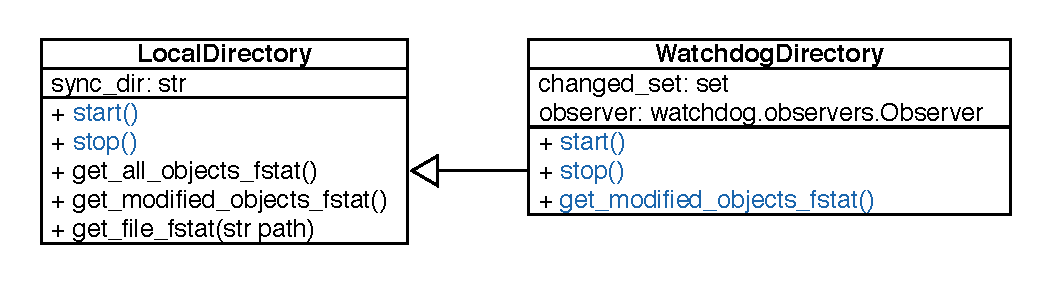
\includegraphics{Images/WatchDir.eps}
    \caption{WatchdogDirectory}
    \label{fig:watchdir_uml}
  \end{figure}

  \begin{itemize}
    \item \textbf{changed\_set}: The set containing all files that were created, modified or renamed, since the last time \emph{get\_modified\_objects\_fstat()} was called.
    \item \textbf{observer}: The thread that monitors the sync directory for changes.\\

    \item \textbf{start}: Starts the observer thread.
    \item \textbf{stop}: Stops the observer thread.
    \item \textbf{get\_modified\_objects\_fstat}: Returns the metadata of the files in the \emph{changed\_set} as FileStat objects. Clears the \emph{changed\_set}.
  \end{itemize}

  \subsection{Benchmarks}
    For this benchmark, we created a directory containing 1.000.000 files (1000 directories of 1000 files each). A LocalDirectory and a WatchdogDirectory instance were created and started and then a number of files were modified. Immidiately afterwards, a list of the modified files was requested and we the response time was timed. Each test was executed 5 times, and the average of the results are shown on the tables \ref{table:mbp-watch}, \ref{table:vm-watch} and graphed on figures \ref{fig:mpb-watch-graph}, \ref{fig:vm-watch-graph}.

    \begin{table}[H]
      \setlength{\tabcolsep}{12pt}
      \begin{adjustbox}{max width=1.2\textwidth, center}
      \begin{tabular}{c|*{7}{c|}c}
        \cline{2-8}
        & \multicolumn{7}{ |c| }{\textbf{\# files modified}} & \\ \cline{2-9}
        & \textbf{0} & \textbf{10} & \textbf{100} & \textbf{1000} & \textbf{10000} & \textbf{100000} & \textbf{1000000} & \multicolumn{1}{|c|}{\textbf{default}}\\ \cline{1-9}
        \multicolumn{1}{|c|}{\textbf{time (s)}} & 1.06E-5 & 0.004 & 0.038 & 0.339 & 1.618 & 12.907 & 90.003 & \multicolumn{1}{|c|}{108.110}\\ \cline{1-9}
        \multicolumn{1}{|c|}{\textbf{speedup (\%)}} & 100.000 & 99.996 & 99.965 & 99.687 & 98.503 & 92.825 & 16.749 & \multicolumn{1}{|c|}{N/A} \\ \cline{1-9}
      \end{tabular}
      \end{adjustbox}
      \caption{MBP local directory \emph{get\_modified\_objects\_fstat()} times, relative to \# of files modified}
      \label{table:mbp-watch}
    \end{table}

    \begin{table}[H]
      \setlength{\tabcolsep}{12pt}
      \begin{adjustbox}{max width=1.2\textwidth, center}
      \begin{tabular}{c|*{7}{c|}c}
        \cline{2-8}
        & \multicolumn{7}{ |c| }{\textbf{\# files modified}} & \\ \cline{2-9}
        & \textbf{0} & \textbf{10} & \textbf{100} & \textbf{1000} & \textbf{10000} & \textbf{100000} & \textbf{1000000} & \multicolumn{1}{|c|}{\textbf{default}}\\ \cline{1-9}
        \multicolumn{1}{|c|}{\textbf{time (s)}} & 9.00E-5 & 5.85E-4 & 0.004 & 0.039 & 0.383 & 4.200 & 41.230 & \multicolumn{1}{|c|}{48.600}\\ \cline{1-9}
        \multicolumn{1}{|c|}{\textbf{speedup (\%)}} & 100.000 & 99.999 & 99.992 & 99.919 & 99.212 & 91.358 & 15.164 & \multicolumn{1}{|c|}{N/A} \\ \cline{1-9}
      \end{tabular}
      \end{adjustbox}
      \caption{VM local directory \emph{get\_modified\_objects\_fstat()} times, relative to \# of files modified}
      \label{table:vm-watch}
    \end{table}

    \begin{figure}[H]
      \centering
      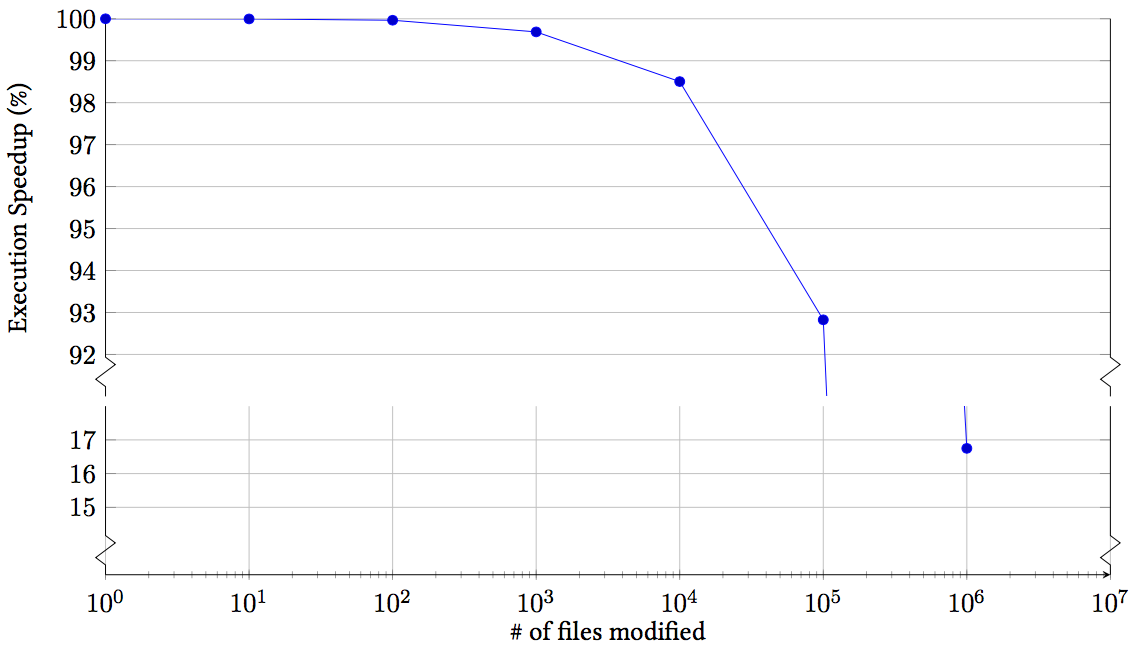
\includegraphics[width=\linewidth]{Images/watchdir-mbp.png}
      \caption{MPB Speedup relative to number of modified files}
      \label{fig:mpb-watch-graph}
        % \begin{tikzpicture}
        %   \begin{groupplot}[
        %       group style={
        %           group name=my plots,
        %           group size=1 by 2,
        %           xticklabels at=edge bottom,
        %           vertical sep=4pt,
        %       },
        %       width=16cm, xmin=1, xmax=1e7
        %   ]
        %   \nextgroupplot[ymin=91,ymax=100,
        %                  ytick={92,...,100},
        %                  axis x line=none,
        %                  axis y discontinuity=crunch,
        %                  height=7cm,
        %                  xmode=log,
        %                  ylabel=Execution Speedup (\%),
        %                  grid=major]
        %     \addplot
        %       coordinates {
        %       (1,100)(1e1,99.996)(1e2,99.965)(1e3,99.687)(1e4,98.503)(1e5,92.825)(1e6,16.749)
        %       };
        %   \nextgroupplot[ymin=13,ymax=18,
        %                  ytick={15,...,17},
        %                  axis x line=bottom,
        %                  axis y discontinuity=crunch,
        %                  height=4cm,
        %                  xmode=log, % xmin=1, xmax=1e7,
        %                  xlabel=\# of files modified,
        %                  grid=major]
        %       \addplot
        %       coordinates {(1e5,92.825)(1e6,16.749)};
        %   \end{groupplot}
        % \end{tikzpicture}
    \end{figure}

    \begin{figure}[H]
      \centering
      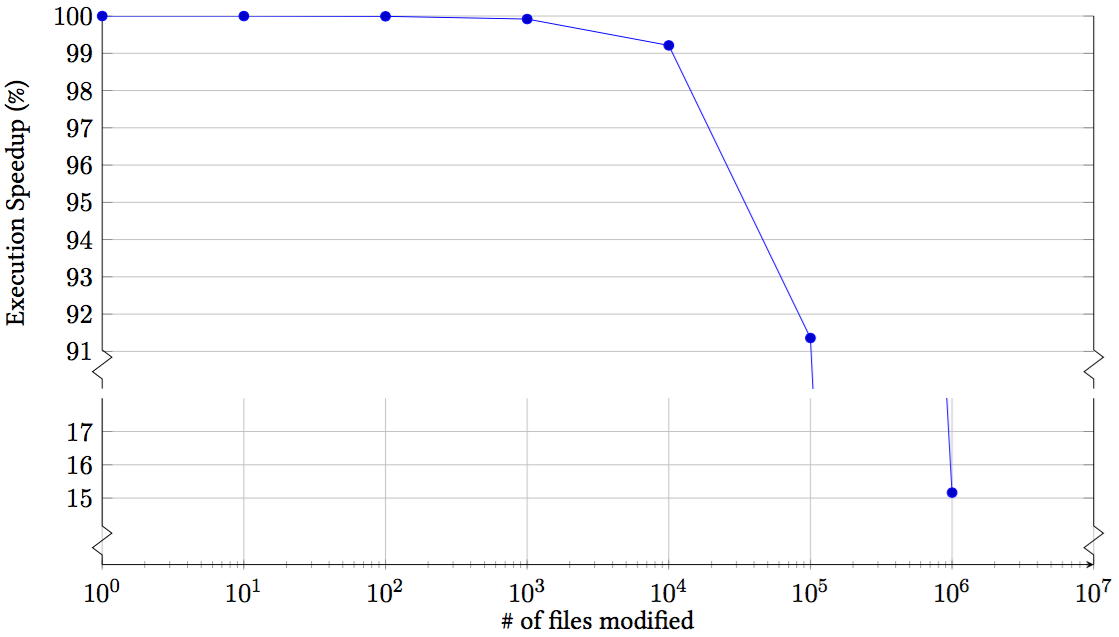
\includegraphics[width=\linewidth]{Images/watchdir-vm.png}
      \caption{VM Speedup relative to number of modified files}
      \label{fig:vm-watch-graph}
        % \begin{tikzpicture}
        %   \begin{groupplot}[
        %       group style={
        %           group name=my plots,
        %           group size=1 by 2,
        %           xticklabels at=edge bottom,
        %           vertical sep=4pt,
        %       },
        %       width=16cm, xmin=1, xmax=1e7
        %   ]
        %   \nextgroupplot[ymin=90,ymax=100,
        %                  ytick={91,...,100},
        %                  axis x line=none,
        %                  axis y discontinuity=crunch,
        %                  height=7cm,
        %                  xmode=log,
        %                  ylabel=Execution Speedup (\%),
        %                  grid=major]
        %     \addplot
        %       coordinates {
        %       (1,100)(1e1,99.999)(1e2,99.992)(1e3,99.919)(1e4,99.212)(1e5,91.358)(1e6,15.164)
        %       };
        %   \nextgroupplot[ymin=13,ymax=18,
        %                  ytick={15,...,17},
        %                  axis x line=bottom,
        %                  axis y discontinuity=crunch,
        %                  height=4cm,
        %                  xmode=log, % xmin=1, xmax=1e7,
        %                  xlabel=\# of files modified,
        %                  grid=major]
        %       \addplot
        %       coordinates {(1e5,91.358)(1e6,15.164)};
        %   \end{groupplot}
        % \end{tikzpicture}
    \end{figure}

    From the results displayed in tables \ref{table:mbp-watch}, \ref{table:vm-watch}, it is obvious that using a directory monitoring mechanism can result in very significant speed gains. This is more apparent in directories with a large number of files; by using this optimisation the time to detect file changes scales linearly with the number of modified files, rather than the total number of files present in the directory.

\section{Local block storage}
  \label{sec:local_block}

  As mentioned before, the motivation behind the creation of this framework was the synchronisation of Virtual Machine images and snapshots. All those files are relatively large in size, usually several GB, and they have many similarities in their data; they are often referred to as \emph{large similar files}. Those similarities can be exploited from local clients in order to improve download speeds, if such a file is already present on the system.

  In this framework, we propose and implement a way to benefit from that characteristic of large similar files. We use a directory on the local filesystem to save the blocks of all the files present in the sync directory. To further improve speed, we take advantage of the caching capabilities of the OS, by creating a structure of 65536 directories, 256 folders containing 256 folders each, named using a hex number from ``00'' to ``ff''. A block is stored at the directory indicated by the first four characters of its hash value. For example, a block with hash value \textbf{abcdef1234567890} would be saved to \textbf{<block\_directory>/ab/cd/ef1234567890}.

  Whenever a file should be downloaded from the remote server, the client first asks for a list containing the hash values of its blocks, and downloads only the ones that do not already exist in the block directory. The file is constructed afterwards, using the stored blocks. To ensure that the block directory contains all the new blocks when a file modification occurs on local, the blocks are stored immediately after a successful object upload or update request at the server. The changes on the CloudClient class are shown in figure \ref{fig:cloud_block_uml}, hilighting the methods that should be modified on derived classes to implement this feature.

  \begin{figure}[!htpb]
    \centering
    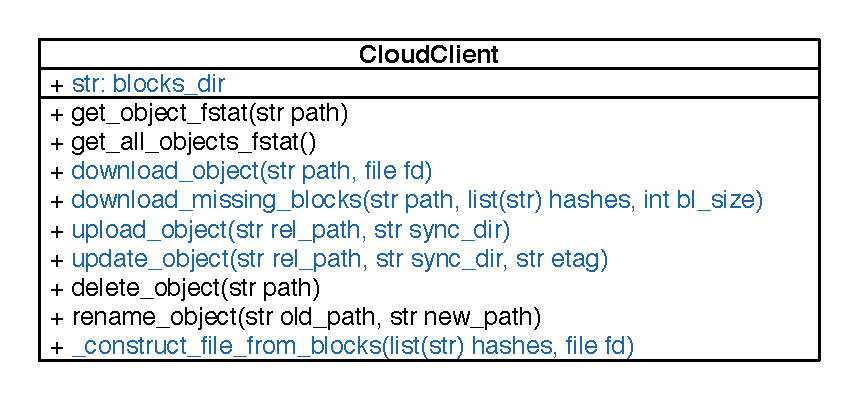
\includegraphics{Images/CloudBlocks.eps}
    \caption{CloudClient with local block storage feature}
    \label{fig:cloud_block_uml}
  \end{figure}

   \begin{itemize}
    \item \textbf{blocks\_dir}: The full path of the directory where file blocks are stored. Optional argument, whose existence denotes the use of the feature.\\

    \item \textbf{download\_object}: Checks the hash list of the remote object and downloads only the blocks that are missing, constructing the file from its hashmap afterwards.
    \item \textbf{download\_missing\_blocks}: Downloads the blocks in `hashes' list that do not already exist on the block directory.
    \item \textbf{upload\_object}: Uploads a file to the remote server and stores its blocks to the block directory.
    \item \textbf{update\_object}: Updates a file at the remote server and stores its blocks to the block directory.
    \item \textbf{\_construct\_file\_from\_blocks}: Static method that constructs and saves a file to the file descriptor `fd', given its hash list `hashes'.
  \end{itemize}

  \subsection{Benchmarks}
  To test the performance of this optimisation, we created a text file of 40 MiB (41,943,040 Bytes) in size which is exactly equal to 10 blocks of 4MiB (4194304 Bytes) each, and uploaded it on the remote server. We then modified some blocks, uploaded the change on the remote, and measured the time needed to download the file. Each benchmark ran five times, the average of which is presented on the results, shown in the table \ref{table:mbp-blockdir} and graphed on figure \ref{fig:mbp-blockdir-graph}.\\

  \begin{table}[H]
    \setlength{\tabcolsep}{12pt}
    \begin{adjustbox}{max width=1.2\textwidth, center}
    \begin{tabular}{c|*{11}{c|}}
      \cline{2-12}
      & \multicolumn{11}{ |c| }{\textbf{\# of modified blocks}}\\ \cline{2-12}
      & \textbf{0} & \textbf{1} & \textbf{2} & \textbf{3} & \textbf{4} & \textbf{5} & \textbf{6} & \textbf{7} & \textbf{8} & \textbf{9} & \multicolumn{1}{|c|}{\textbf{10}}\\ \cline{1-12}
      \multicolumn{1}{|c|}{\textbf{time (s)}} & 0.37 & 2.59 & 4.49 & 6.44 & 8.98 & 10.12 & 12.23 & 13.60 & 15.65 & 17.59 & 19.61 \\ \cline{1-12}
      \multicolumn{1}{|c|}{\textbf{speedup (\%)}} & 98.1 & 86.8 & 77.1 & 67.2 & 54.2 & 48.4 & 37.7 & 30.7 & 20.2 & 10.3 & N/A \\ \cline{1-12}
    \end{tabular}
    \end{adjustbox}
    \caption{MBP file download times, relative to \# of modified blocks}
    \label{table:mbp-blockdir}
  \end{table}

  \begin{figure}[!htpb]
    \centering
    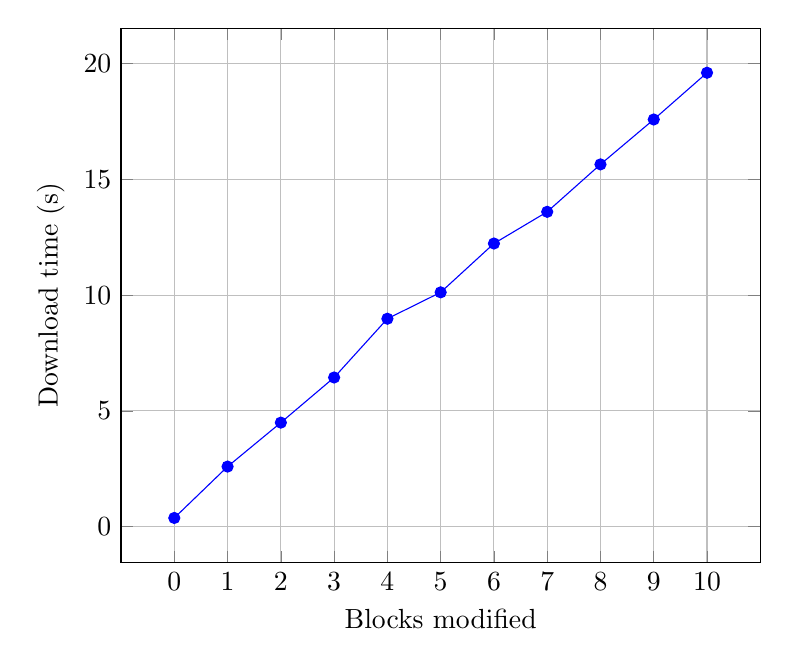
\begin{tikzpicture}
      \begin{axis}[xlabel=Blocks modified, xtick={0,...,10}, ylabel=Download time (s), grid=major, width=0.8\linewidth]
        \addplot[color=blue,mark=*] coordinates {
          (0,0.37) (1,2.59) (2,4.49) (3,6.44) (4,8.98) (5,10.12) (6,12.23) (7,13.60) (8,15.65) (9,17.59) (10,19.61)
        };
      \end{axis}%
    \end{tikzpicture}%
    \caption{MBP file download times, relative to \# of modified blocks}
    \label{fig:mbp-blockdir-graph}
  \end{figure}

  We can see from figure \ref{fig:mbp-blockdir-graph} that the results of the benchmarks very closely approximate a linear correlation. Therefore, the results confirm the hypothesis that the the time needed to download a file is proportional to the number of the blocks that do not exist in the local block directory (and hence, have to be downloaded). This is very important for the main use case that this framework was created for, since it allows considerably faster downloads of large similar files. The performance gain achieved on a file download by this optimisation is approximately:

  \[\textrm{Performance gain \%} = \left(1 - \frac{\textrm{\# of new blocks}}{\textrm{Total \# of blocks}} \right) \times 100\]

  % TODO: Limitation: aligned blocks

\section{Local deduplication - FUSE}
  \label{sec:fuse}
  As mentioned on section \ref{sec:local_block}, we can implement local block storage, to improve download speeds for large similar files. Even using this method, storing many VM snapshots or images requires large amounts of disk space, since the files are being constructed from their blocks, taking space in the file system. Since those files consist of a significant amount of same blocks, very efficient data compression can be achieved by using deduplication techniques on the local file system.

  The solution proposed is to only store the blocks in the block directory and not reconstruct the files in the syncing directory, but link a file's hash list to the corresponding blocks in the block directory instead. This solution requires modifications to most existing file systems, so either a kernel module or a Filesystem in Userspace (FUSE) mechanism is required, of which we propose the latter. This mechanism should modify the calls to \emph{fstat(), open(), read()} and \emph{write()} system calls, to use the blocks a file is consisted of. The design should follow the ``\emph{Write once, Read many, Update never}'' practice, which suggests never modifying a block in the block directory, but instead use the Copy on Write (CoW) strategy, to create new blocks when changes are required. This ensures that the original resources remain unchanged on the disk, so different files sharing this block will not get corrupted.

  This method effectively implements deduplication on the local file system, reducing storage space required by approximately
  \[block\_size \times \sum_{i=1}^{n}\left[{(\textrm{\# of files sharing block i} - 1}\right]\]
  which can be a significant amount of space, when storing large similar files.

  Apart from the space reduction, a FUSE mechanism implementation provides additional benefits for a file synchronisation framework. File copying within the directory managed by FUSE becomes a very fast and computationaly light procedure, since only a file's hash list needs to be copied to the new location. Furthermore, this optimisation works well in tandem with the file monitoring optimisation described in section \ref{sec:dir_monitoring}. Being in control of the filesystem means we are able to immediately detect changes to files and process only those during the synchronisation. At the time of writing, the FUSE mechanism has been extensively design, but not yet implemented.
